% !TEX program = xelatex
\documentclass[11pt]{beamer}

\usepackage{unicode-math}
\usepackage{amsmath}
\usepackage{amsfonts}
\usepackage{amssymb}
\usepackage[style=ddmmyyyy]{datetime2}
\usepackage{graphicx}
\usepackage{hyperref}
\usepackage{fontspec}
\usepackage[dvipsnames]{xcolor}
\usepackage{tikz}
\usepackage{soul}
\usepackage{ulem}

\makeatletter
\def\input@path{{../../theme/}}
\def\beamer@shrinkfactorinv{1}
\makeatother

%beamer setup
\usetheme[subsectionpage=progressbar]{mis}
\setbeamerfont{caption}{size=\footnotesize}
\setsansfont{Lato}[Numbers=OldStyle]
\setmathfont{STIX Two Math}[Scale=MatchLowercase]
\setmonofont{Consolas}[Scale=MatchLowercase]

%tikz 
\usetikzlibrary{calc} 
\usetikzlibrary{arrows, decorations.markings, positioning, backgrounds, shapes}
\definecolor{EMP}{HTML}{77DD77} % Green1
\definecolor{NOR}{HTML}{06500C} % Green2
%tikz settings
\renewcommand{\ULdepth}{3pt}
\tikzset{
  EMP/.style={% Style for empatized boxes
      rectangle, line width=1pt,
      anchor=west,
      %underline, % new property
      align=center,
      text=Black,
      minimum height=.8cm,
      text height=1.25ex,
          text depth=.25ex,
      fill=EMP,
      draw=black,
  },
  NOR/.style={% Style for normal boxes.
      rectangle, 
      line width=1pt,
      anchor=west,
      align=left,
      minimum height=.6cm,
      text height=1.25ex,
          text depth=.25ex,
          text=white,
      fill=NOR,
      draw=black,
      inner ysep=5pt
  },
  fkey/.style={
    to path={
      ([xshift={\sourcedown*(-1ex)}]\tikztostart)
      |- ([xshift={\relationright+\sourcedown*(-1ex)},yshift={\sourcedown*(-1ex)-2ex}]\tikztostart)
      |- ([yshift={\targetdown*(-1ex)-2ex},xshift={\targetdown*(-1ex)}]\tikztotarget)
      -- ([xshift={\targetdown*(-1ex)}]\tikztotarget)
    },
    ->,>=latex,
    relation/.cd,#1
  },
  relation/.cd,
  source/.store in=\sourcedown,
  source = 0,
  target/.store in=\targetdown,
  target = 0,
  right/.store in=\relationright,
  right = 1 cm
}
\def\relation(#1)#2[#3]#4{%
  \begin{scope}[shift={(#1)}] 
      \node[font=\bf, anchor=west] (Title) at (-0.25,0.75) {#3}; 
       \edef\k{0}% Variable for box positión
       \edef\x{0}% Variable for named coordinate centering - below box
       \foreach \id/\style in {#4} {%enter sub frame data Name/Boxtype ,Name2/Boxtype | An space before Boxtype is needed 
            \node[\style] (h) at (\k pt,0) {\id}; %  % Draw a node depending on the variables.
            \pgfmathparse{\k+0.5*width{"\id"}+3.4pt} % Uses the textwidth to calculate named coordinate  
            \xdef\x{\pgfmathresult} % The resul is saved in the variable \x
            \draw (\x pt,-0.4) coordinate (\id#2); %Create a named coordinate concatenated: "sub frame data Name"+"identifier"
            \pgfmathparse{\k+width{"\id"}+6.8pt}% Calculate positión for each subframe box.       
        \xdef\k{\pgfmathresult}% Save the value to be added to the next iteration value.
       }    
  \end{scope}
}

\author{Lê Thành Văn}
\title{Các dạng chuẩn của CSDL quan hệ}
\institute{Khoa Hệ thống thông tin quản lý}
\date{\today}
\hypersetup {
	colorlinks = true
}
%\usecolortheme{seahorse}
% graphic path
\graphicspath{{../../media/}}

\renewcommand{\figurename}{Hình}
\newcommand{\fd}[2]{#1 \rightarrow #2}%
%
\AtBeginSection{
  \frame{
    \sectionpage
  }
}
\begin{document}
\begin{frame}
  \titlepage
\end{frame}

\section{Giới thiệu}
\subsection{Định nghĩa}
\begin{frame}
  Chuẩn hóa cơ sở dữ liệu (csdl) là quá trình tách bảng dữ liệu nhằm:
  \begin{itemize}
    \item giảm thiểu việc dư thừa dữ liệu, và
    \item hạn chế lỗi có thể phát sinh trong quá trình thay đổi dữ liệu.
  \end{itemize}
\end{frame}

\begin{frame}
  Việc chuẩn hóa csdl dựa trên các dạng chuẩn (normal form) được Edgar F. Codd
  đề ra trong mô hình quan hệ của mình.
\end{frame}
\subsection{Các loại lỗi}
\begin{frame}
  \textbf{Lỗi khi thay đổi dữ liệu} (thêm, sửa hoặc xóa) là dạng lỗi khi dữ liệu được thay đổi không tương thích 
  với cấu trúc hoặc dữ liệu hiện có.
\end{frame}

\begin{frame}
  Giả sử thông tin giảng viên \textit{cần} bao gồm mã môn học họ giảng dạy.
  Tuy nhiên, một giảng viên mới có thể chưa có môn, dẫn đến không thể thêm thông tin của họ.

  \begin{figure}
    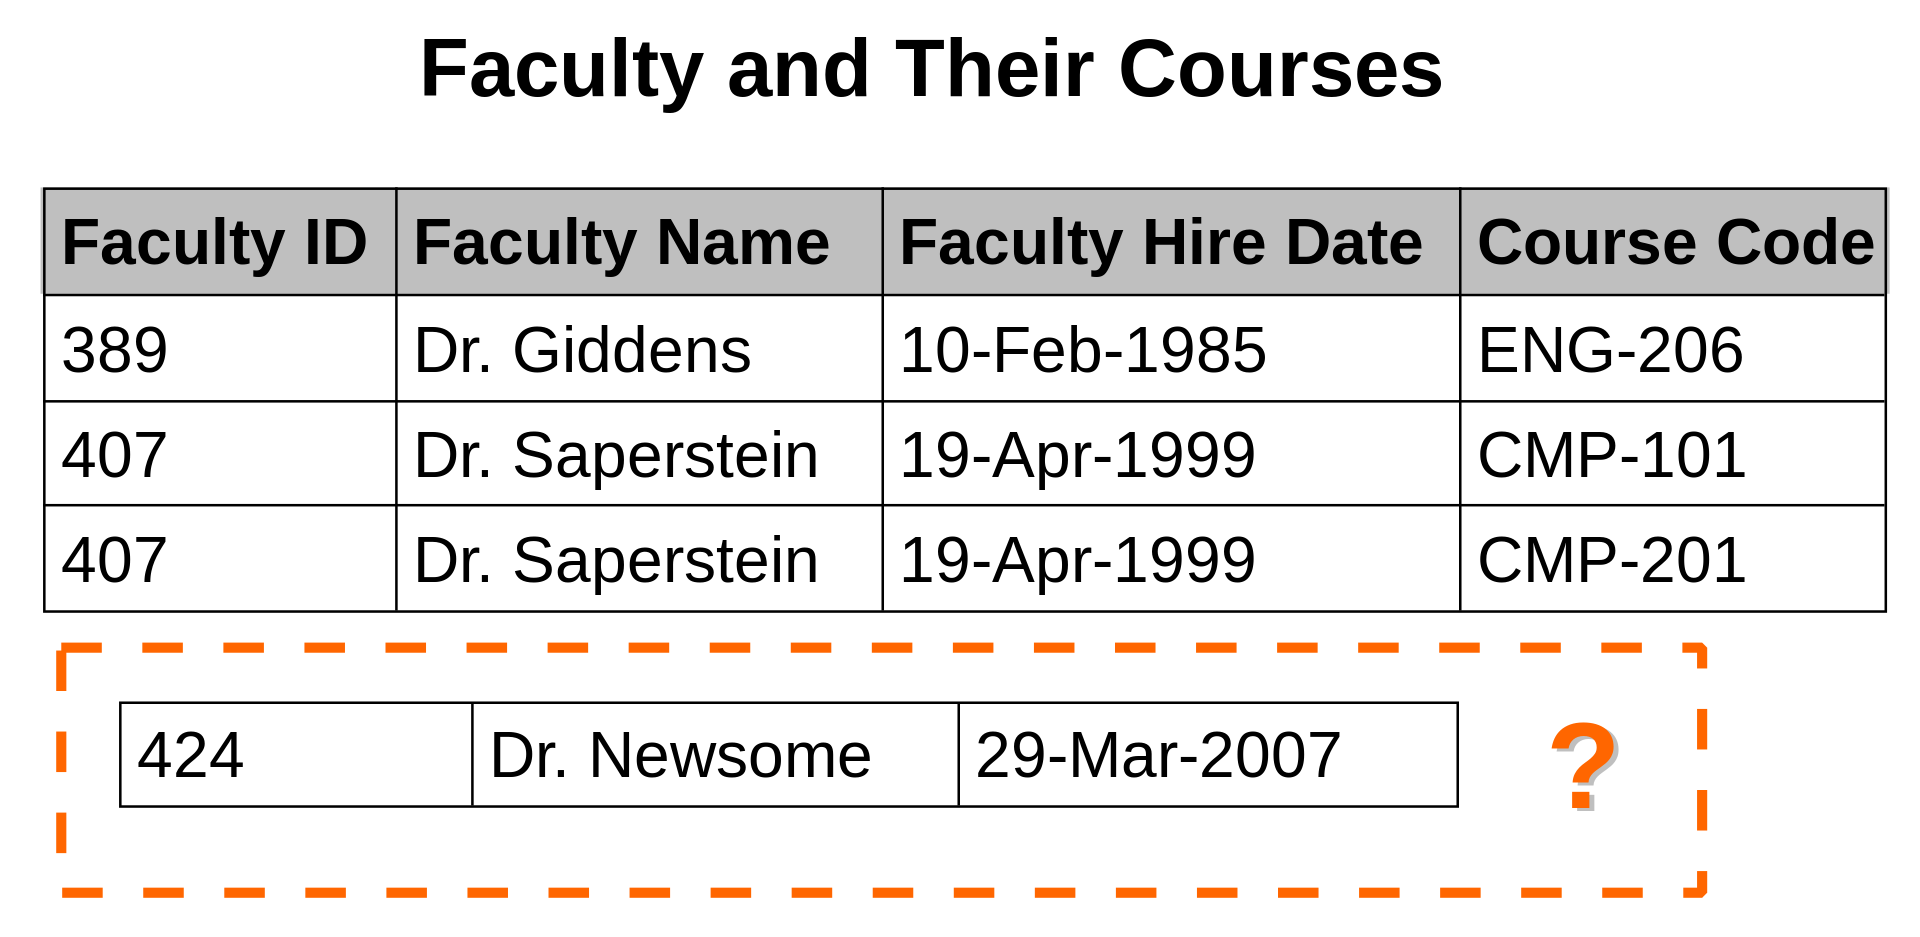
\includegraphics[width=0.75\textwidth]{COS212/ia.png}
    \caption{\textit{Lỗi khi thêm dữ liệu}}
  \end{figure}
\end{frame}

\begin{frame}
  Một thông tin có thể xuất hiện nhiều lần trong một bảng, nên khi thay đổi có thể bị sót, 
  dẫn đến thông tin không nhất quán trong csdl.
  \begin{figure}
    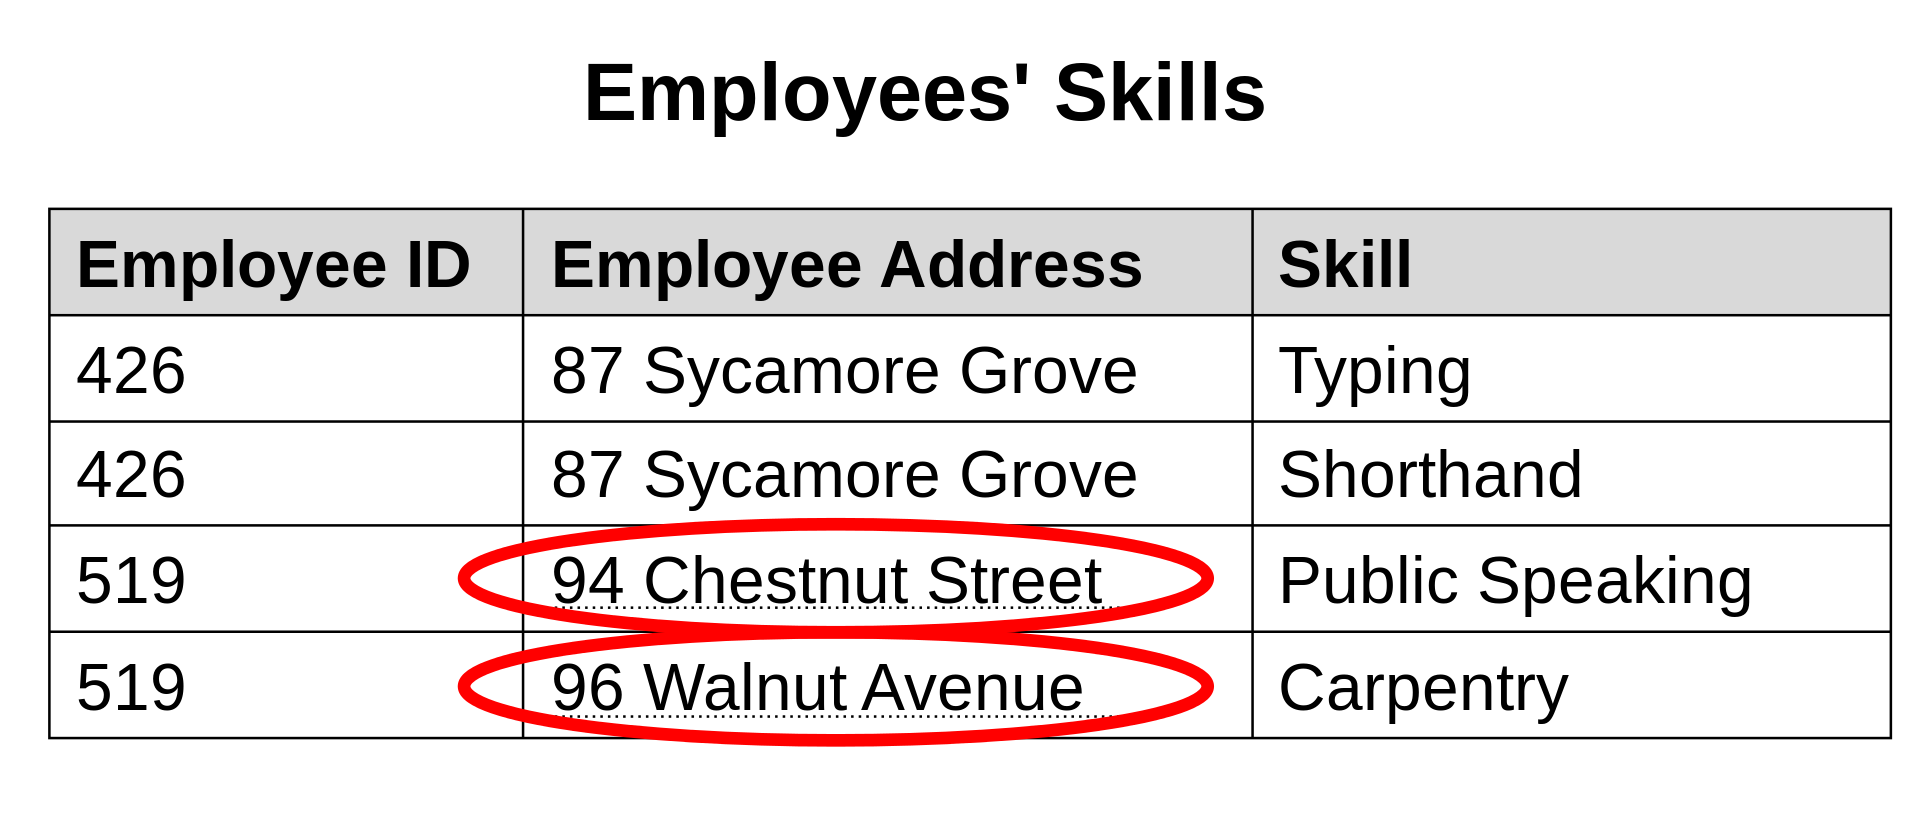
\includegraphics[width=0.75\textwidth]{COS212/ua.png}
    \caption{\textit{Lỗi khi sửa dữ liệu}}
  \end{figure}
\end{frame}

\begin{frame}
  Lỗi khi xóa dữ liệu là dạng lỗi mà khi xóa một thông tin này có thể xóa những 
  thông tin (không cần xóa) khác.
  \begin{figure}
    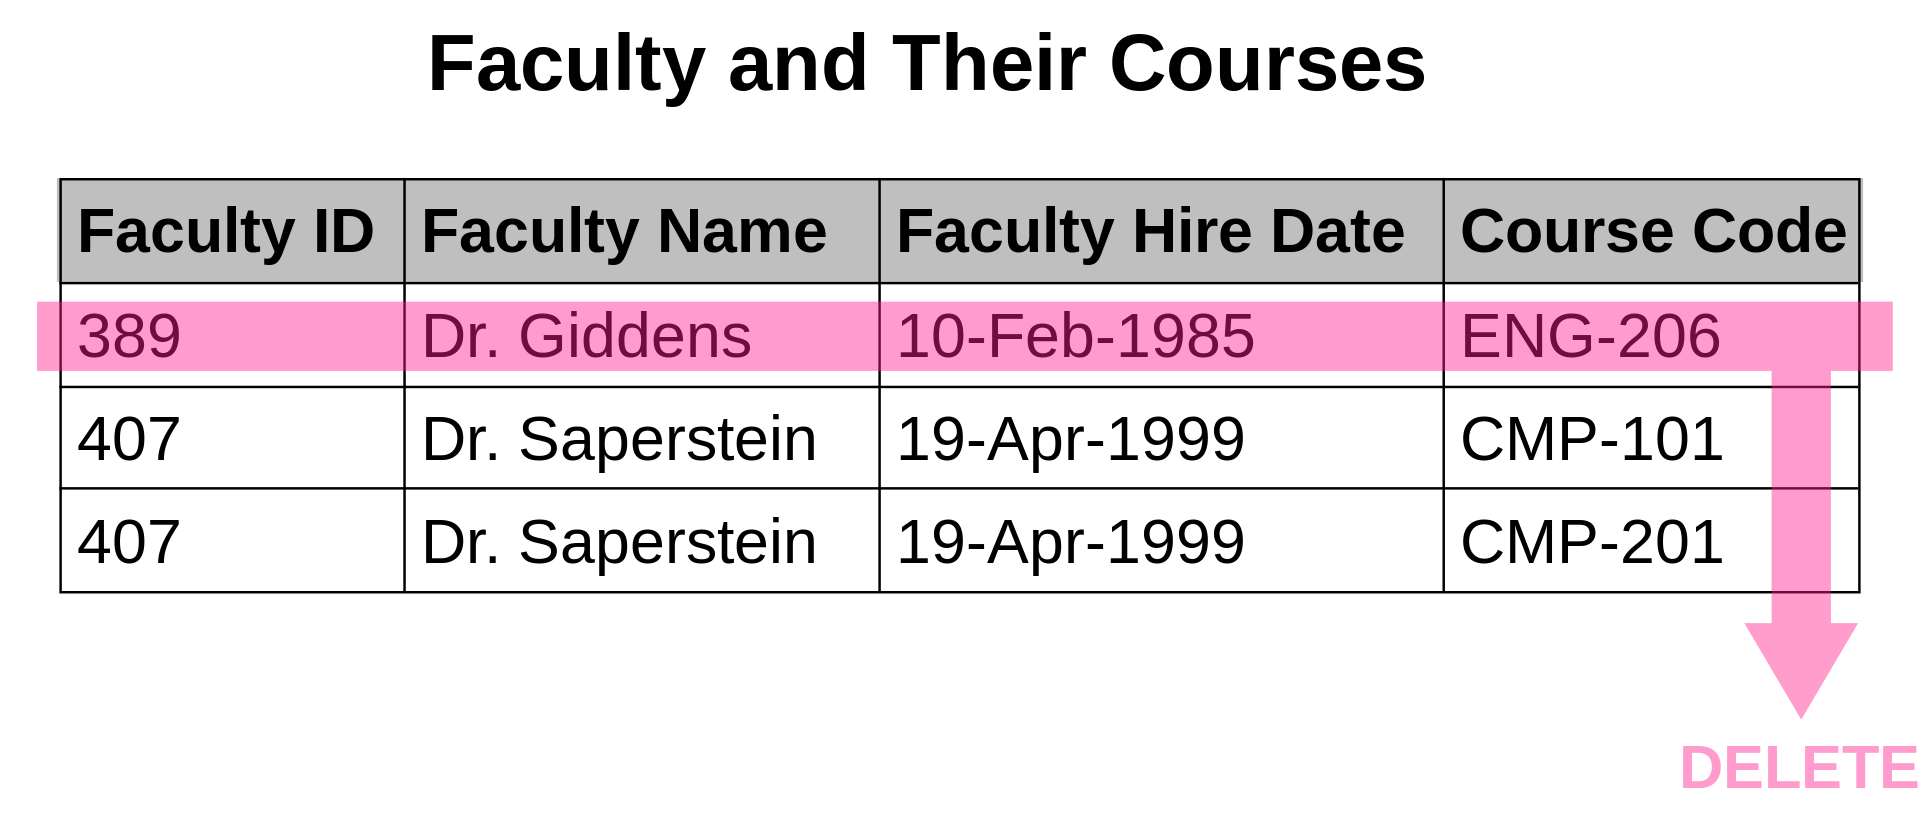
\includegraphics[width=0.75\textwidth]{COS212/da.png}
    \caption{\textit{Lỗi khi xóa dữ liệu}}
  \end{figure}
\end{frame}

\subsection{Các dạng chuẩn}
\begin{frame}
  Các dạng chuẩn thường gặp bao gồm (từ thấp đến cao):
  \begin{itemize}
    \item Dạng chuẩn 1 (First Normal Form, 1NF).
    \item Dạng chuẩn 2 (Second Normal Form, 2NF).
    \item Dạng chuẩn 3 (Third Normal Form, 3NF).
    \item Dạng chuẩn Boyce-Codd (Boyce-Codd Normal Form, BCNF, 3.5NF). 
  \end{itemize}
\end{frame}

\begin{frame}
  Việc đạt được một dạng chuẩn cao có nghĩa là phải thỏa mãn điều kiện của các dạng chuẩn thấp hơn nó.\\
  Tức là, không thể đạt được dạng chuẩn 3 nếu như không đạt được dạng chuẩn 1 hoặc dạng chuẩn 2.
\end{frame}

\begin{frame}
  Một csdl quan hệ được gọi là \textbf{đã chuẩn hóa} nếu như nó đạt được dạng chuẩn 3.
\end{frame}

\section{Các dạng chuẩn}
\begin{frame}
  Chúng ta sẽ dùng dữ liệu sau đây để tìm hiểu về các dạng chuẩn cũng như quá trình chuẩn hóa csdl.
  \begin{figure}
    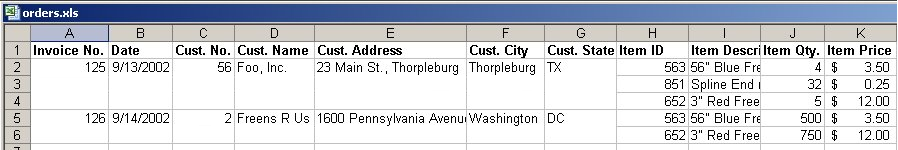
\includegraphics[width=\textwidth]{COS212/un.png}
    \caption{\textit{CSDL chưa chuẩn hóa}}
  \end{figure}
\end{frame}

\subsection{Dạng chuẩn 1}
\begin{frame}
  \textbf{Dạng chuẩn 1} đạt được khi giá trị của mỗi ô là nguyên tố, tức là
  không thể chia nhỏ giá trị đó thành nhiều phần có ý nghĩa tương đương.
\end{frame}

\begin{frame}
  Để đưa cơ sở dữ liệu về dạng chuẩn 1, chúng ta cần tách các giá trị không nguyên tố 
  thành từng dòng riêng biệt.
  \begin{figure}
    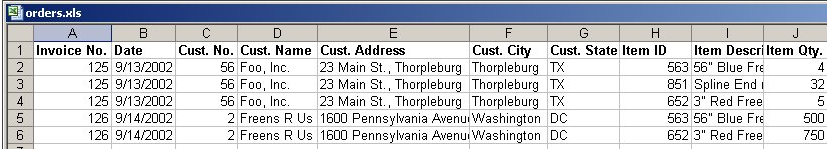
\includegraphics[width=\textwidth]{COS212/1nf.png}
    \caption{\textit{CSDL đạt dạng chuẩn 1}}
  \end{figure}
\end{frame}

\begin{frame}
  Hoặc là cũng có thể tách các giá trị không nguyên tố thành bảng riêng,
  kèm với một khóa ngoại tham chiếu đến bảng cũ.
  \begin{tikzpicture}
    \relation(0, 0){1}[INVOICE]{
      InvNo/EMP,
      Date/NOR,
      CusNo/NOR,
      CusName/NOR,
      CusAddr/NOR,
      CusCity/NOR,
    }
    \relation(0, -2.5){2}[INVOICE-ITEM]{
      ItemId/EMP,
      InvNo/EMP,
      ItemDesc/NOR,
      ItemQuan/NOR,
      ItemPrice/NOR,
    }
    \draw[thick] 
      (InvNo2) edge[fkey={right=-2.5cm}] (InvNo1);
  \end{tikzpicture}
\end{frame}
\subsection{Phụ thuộc hàm}
\begin{frame}
  Để hiểu về dạng chuẩn 2, chúng ta cần đến khái niệm phụ thuộc hàm.\\
  \textit{Định nghĩa}. Cho quan hệ $R(X, Y, ...)$, ta nói $Y$ phụ thuộc vào $X$ nếu như
  khi biết được giá trị của $X$ thì ta xác định được \textbf{một} giá trị duy nhất của $Y$. \\
  Ký hiệu: $X \rightarrow Y$, đọc là $X$ xác định $Y$ hoặc $Y$ phụ thuộc vào $X$.  
\end{frame}

\begin{frame}
  \begin{columns}
    \begin{column}{0.5\textwidth}
      Với dữ liệu ở bảng bên, ta có thể thấy các phụ thuộc hàm sau:
      \begin{itemize}
        \item<1-> $\fd{A}{B}$, $\fd{A}{C}$, \dots
        \item<2-> $\fd{BC}{A}$, $\fd{BC}{DE}$
        \item<3-> \dots
      \end{itemize}
    \end{column}
    \begin{column}{0.5\textwidth}
      \begin{tabular}{|c|c|c|c|c|}
        \hline
        \textbf{A} & \textbf{B} & \textbf{C} & \textbf{D} & \textbf{E} \\
        \hline
        a1 & b1 & c1 & d1 & e1 \\
        \hline
        a2 & b1 & c2 & d2 & e1 \\
        \hline
        a3 & b2 & c1 & d1 & e1 \\
        \hline
        a4 & b2 & c2 & d2 & e1 \\
        \hline
        a5 & b3 & c3 & d1 & e1 \\
        \hline
      \end{tabular}
    \end{column}
  \end{columns}
\end{frame}

\begin{frame}
  Cho quan hệ $R(X, Y, Z)$, phụ thuộc hàm có một số tính chất:
  \begin{itemize}
    \item \textbf{Tính phản xạ}. $\fd{XY}{X}$.
    \item \textbf{Tính tăng trưởng}. Nếu $\fd{X}{Y}$ thì $\fd{XZ}{YZ}$.
    \item \textbf{Tính bắc cầu}. Nếu $\fd{X}{Y}$ và $\fd{Y}{Z}$ thì $\fd{X}{Z}$.
  \end{itemize}
  \textbf{Câu hỏi}. Chứng minh nếu $\fd{X}{Y}$ và $\fd{X}{Z}$ thì $\fd{X}{YZ}$.
\end{frame}

\begin{frame}
  \begin{proof}[Chứng minh]
    \begin{enumerate}
      \item<1-> $\fd{X}{Z} \Rightarrow \fd{X}{XZ}$ (tính tăng trưởng).
      \item<2-> $\fd{X}{Y} \Rightarrow \fd{XZ}{YZ}$ (tính tăng trưởng).
      \item<3-> Dùng tính bắt cầu từ 2 điều trên, ta có $\fd{X}{YZ}$.
    \end{enumerate}
  \end{proof}
\end{frame}
\subsection{Dạng chuẩn 2}
\begin{frame}
  \textbf{Dạng chuẩn 2} đạt được khi:
  \begin{itemize}
    \item Đạt được dạng chuẩn 1.
    \item Không tồn tại phụ thuộc hàm một phần đối với bất kỳ khóa ứng viên có trong bảng.
  \end{itemize}
\end{frame}
\begin{frame}
  Điều kiện thứ hai có nghĩa là, với bất kỳ khóa ứng viên có nhiều hơn hai cột, giả sử là $XY$,
  thì với bất kỳ cột $Z$ không tham gia khóa, ta \textbf{chỉ có} $\fd{XY}{Z}$, 
  mà không có $\fd{X}{Z}$ hoặc $\fd{Y}{Z}$.
\end{frame}
\begin{frame}
  Nhắc lại:
  \begin{itemize}
    \item \textbf{Siêu khóa} là tập hợp một hay nhiều cột có tác dụng xác định một bộ duy nhất khi biết giá trị của siêu khóa.
    \item \textbf{Khóa ứng viên} là siêu khóa, nhưng khi bỏ bất kỳ cột nào trong khóa ứng viên thì nó không còn là siêu khóa nữa.
  \end{itemize}
\end{frame}
\begin{frame}
  Từ định nghĩa trên, có thể thấy rằng trong bảng \textbf{INVOICE-ITEM} có khóa ứng viên là
  \{ItemId, InvNo\}.
  \begin{tikzpicture}
    \relation(0, 0){1}[INVOICE-ITEM]{
      ItemId/EMP,
      InvNo/EMP,
      ItemDesc/NOR,
      ItemQuan/NOR,
      ItemPrice/NOR,
    }
  \end{tikzpicture}
  \newline
  Bây giờ, để tìm những cột không thỏa dạng chuẩn 2, ta cần trả lời câu hỏi 
  \textit{`Có thể biết được thông tin này mà không cần biết toàn bộ \{ItemId, InvNo\} hay không?'}
  cho từng cột.
\end{frame}
\begin{frame}
  Có thể thấy được rằng:
  \begin{itemize}
    \item<1-> Cột ItemQuan phụ thuộc vào \{ItemId, InvNo\}.
    \item<2-> Cột ItemDesc và ItemPrice chỉ phụ thuộc vào ItemId.
  \end{itemize}
  \uncover<3->{Vì vậy, bảng này không đạt dạng chuẩn 2.}
\end{frame}
\begin{frame}
  \uncover<1->{Việc cần làm là tách những cột phụ thuộc một phần cùng với cột xác định của chúng 
  thành một quan hệ mới.\\}
  \uncover<2->{Cột xác định trong bảng cũ sẽ thành khóa ngoại tham chiếu đến bảng vừa tách.}
\end{frame}
\begin{frame}
  Áp dụng quy tắc trên, ta được csdl mới như sau:
  \begin{tikzpicture}
    \relation(0, 0){1}[INVOICE]{
      InvNo/EMP,
      Date/NOR,
      CusNo/NOR,
      CusName/NOR,
      CusAddr/NOR,
      CusCity/NOR,
    }
    \relation(0, -2){2}[INVOICE-ITEM]{
      ItemId/EMP,
      InvNo/EMP,
      ItemQuan/NOR,
    }
    \relation(0, -4){3}[ITEM]{
      ItemId/EMP,
      ItemDesc/NOR,
      ItemPrice/NOR,
    }
    \draw[thick] 
      (InvNo2) edge[fkey={right=-2.5cm}] (InvNo1)
      (ItemId2) edge[fkey={right=5cm, source=1}] (ItemId3);
  \end{tikzpicture}
\end{frame}
\begin{frame}
  Ngoài ra, có thể thấy trong bảng \textbf{INVOICE}, bên cạnh việc cột InvNo có thể xác định được
  CusName, CusAddr, CusCity, các cột đó cũng phụ thuộc vào CusNo.
\end{frame}
\begin{frame}
  Từ đó, ta có phụ thuộc hàm bắc cầu InvNo $\rightarrow$ CusNo $\rightarrow$ \{CusName, CusAddr, CusCity\}.\\
  Trong dạng chuẩn 3, chúng ta sẽ làm việc với những phụ thuộc hàm bắc cầu này.
\end{frame}
\subsection{Dạng chuẩn 3}
\begin{frame}
  \uncover<1->{\textbf{Dạng chuẩn 3} đạt được khi:}
  \begin{enumerate}
    \item<2-> Đạt được dạng chuẩn 2.
    \item<3-> Không tồn tại phụ thuộc hàm bắt cầu.
  \end{enumerate}
\end{frame}
\begin{frame}
  \uncover<1->{Tương tự cách đưa về dạng chuẩn 2, để đưa về dạng chuẩn 3:}
  \begin{enumerate}
    \item<2-> Tách các cột phụ thuộc bắc cầu cùng cột (không phải khóa) xác định chúng thành bảng riêng.
    \item<3-> Thêm khóa ngoại cho bảng được tách tham chiếu đến bảng vừa tạo.
  \end{enumerate}
\end{frame}
\begin{frame}  
  \uncover<1->{Áp dụng quy tắc trên, ta được csdl mới như sau:}
  \uncover<2->{
    \begin{tikzpicture}
    \relation(0, 0){1}[INVOICE]{
      InvNo/EMP,
      Date/NOR,
      CusNo/NOR,
    }
    \relation(0, -2){2}[CUSTOMER]{
      CusNo/EMP,
      CusName/NOR,
      CusAddr/NOR,
      CusCity/NOR,
    }
    \relation(0, -4){3}[INVOICE-ITEM]{
      ItemId/EMP,
      InvNo/EMP,
      ItemQuan/NOR,
    }
    \relation(5, -4){4}[ITEM]{
      ItemId/EMP,
      ItemDesc/NOR,
      ItemPrice/NOR,
    }
    \draw[thick] 
      (InvNo3) edge[fkey={right=-2.5cm, source=-1}] (InvNo1)
      (CusNo1) edge [fkey={right=5cm}] (CusNo2);
    \draw[thick, ->, thick, >=latex]
      (ItemId3) |- ++(0.5ex, -2.5ex) -| (ItemId4);      
  \end{tikzpicture}
  }
\end{frame}
\begin{frame}
  Trong một số trường hợp, dạng chuẩn 3 là chưa đủ để tránh khỏi lỗi trong quá trình thay đổi dữ liệu.
\end{frame}
\begin{frame}
  Cùng xem ví dụ sau:
  \begin{itemize}
    \item Một sinh viên có thể có nhiều chuyên ngành.
    \item Với mỗi chuyên ngành của mình, sinh viên có đúng một người hướng dẫn.
    \item Mỗi chuyên ngành có nhiều người hướng dẫn.
    \item Mỗi người hướng dẫn chỉ hướng dẫn một chuyên ngành.
    \item Mỗi người hướng dẫn có thể hướng dẫn nhiều sinh viên.
  \end{itemize}
\end{frame}
\begin{frame}
  \begin{tikzpicture}
    \relation(0, 0)[HƯỚNG DẪN]{
      mã sinh viên/EMP,
      chuyên ngành/EMP,
      người hướng dẫn/NOR,
    }
  \end{tikzpicture} \\
  Chúng ta có các phụ thuộc hàm:
  \begin{enumerate}
    \item \{\textit{mã sinh viên, chuyên ngành}\} $\rightarrow$ \textit{người hướng dẫn}.
    \item \{\textit{mã sinh viên, người hướng dẫn}\} $\rightarrow$ \textit{chuyên ngành}.
    \item \textit{người hướng dẫn} $\rightarrow$ \textit{chuyên ngành}.
  \end{enumerate}
\end{frame}
\begin{frame}
  \uncover<1->{Bảng này tuy đạt dạng chuẩn 3, nhưng vẫn có những lỗi xảy ra khi thay đổi dữ liệu:}
  \begin{itemize}
    \item<2-> \textbf{Thêm dữ liệu}: Thêm người hướng dẫn mới cần có sinh viên.
    \item<3-> \textbf{Cập nhật dữ liệu}: Có thể không nhất quán.
    \item<4-> \textbf{Xóa dữ liệu}: Xóa thông tin sinh viên có thể làm mất thông tin người hướng dẫn.
  \end{itemize}
\end{frame}
\begin{frame}
  Để giải quyết, chúng ta cần tách bảng để đạt được dạng chuẩn Boyce-Codd.
\end{frame}
\subsection{Dạng chuẩn Boyce-Codd}
\begin{frame}
  \uncover<1->{\textbf{Dạng chuẩn Boyce-Codd} đạt được khi:}
  \begin{enumerate}
    \item<2-> Đạt được dạng chuẩn 3.
    \item<3-> Với bất kỳ phụ thuộc hàm $\fd{X}{Y}$ thì $X$ phải là siêu khóa.
  \end{enumerate}
\end{frame}
\begin{frame}
  Có thể thấy được rằng, ví dụ \textbf{HƯỚNG DẪN} ở trên không đạt dạng chuẩn Boyce-Codd 
  do có phụ thuộc hàm \textit{người hướng dẫn} $\rightarrow$ \textit{chuyên ngành}.
\end{frame}
\begin{frame}
  Vi phạm dạng chuẩn Boyce-Codd thường xuất hiện khi một bản có nhiều khóa ứng viên
  và các khóa này có một hoặc nhiều cột giống nhau.
\end{frame}
\begin{frame}
  \uncover<1->{Để đưa về dạng chuẩn Boyce-Codd:}
  \begin{enumerate}
    \item<2-> Tách các phụ thuộc hàm vi phạm dạng chuẩn Boyce-Codd thành bảng riêng.
    \item<3-> Thêm khóa ngoại cho bảng được tách tham chiếu đến bảng vừa tạo.
  \end{enumerate}
\end{frame}
\begin{frame}
  \uncover<1->{Áp dụng quy trình trên, ta được}
  \uncover<2->{
    \begin{tikzpicture}
      \relation(0, 0){1}[HƯỚNG DẪN SINH VIÊN]{
        mã sinh viên/EMP,
        người hướng dẫn/EMP,
      }
      \relation(0, -2){2}[HƯỚNG DẪN CHUYÊN NGÀNH]{
        người hướng dẫn/EMP,
        chuyên ngành/NOR,
      }
      \draw[thick]
      (người hướng dẫn2) edge[fkey={right=5cm}] (người hướng dẫn1); 
    \end{tikzpicture}
  }
\end{frame}
\section{Quy trình chuẩn hóa}
\begin{frame}
  \uncover<1->{Như có thể thấy, quy trình chuẩn hóa có thể tóm gọn như sau:}
  \begin{enumerate}
    \item<2-> Xác dịnh các cột không nguyên tố để đưa về dạng chuẩn 1.
    \item<3-> Xác định các phụ thuộc hàm.
    \item<4-> Tách bảng dựa trên phụ thuộc hàm.
  \end{enumerate}
\end{frame}
\end{document}